\chapter{Evaluation}
\label{chap:evaluation}

\begin{introduction}

A series of experiments was designed and conducted in a controlled environment to rigorously assess the performance, resilience, and modularity of the proposed Resilient Federated Learning Framework. This chapter details the experimental setup, the datasets and models used, the metrics measured, the various experimental scenarios investigated, and the results and analysis for each scenario.

\end{introduction}

\section{Experimental Setup}
\label{sec:experimental-setup}

The experimental setup was designed to emulate scenarios involving resource-constrained client devices participating in a federated training process coordinated by a more powerful central server. This mirrors typical edge computing \ac{fl} use cases where client devices (like mobile phones or \ac{iot} devices) have limited computational resources and unstable network connectivity compared to a central server or cloud instance. 

The experiments were conducted on a cluster of \acp{vm} running on underlying ARM-based hardware, specifically the HUAWEI Kunpeng 920 7260 processor\footnote{\url{https://www.hisilicon.com/en/products/kunpeng/huawei-kunpeng/huawei-kunpeng-920}},  with Ubuntu 24.04 LTS as the guest operating system. This cluster was hosted on a Proxmox server, which provided a flexible and efficient virtualization environment. 

The cluster configuration for the experiments included a single \ac{vm} designated as the Parameter Server, configured with 8 CPU cores and 16 GB of RAM, providing significantly more resources than the worker \acp{vm}, and with a network interface configured with a maximum bandwidth of approximately 5 GBps, simulating a high-capacity central node connection. This configuration ensured that the Parameter Server could handle the computational load of aggregation and avoid becoming a network bottleneck, allowing us to focus on communication challenges between the server and the workers.

To represent different client populations, two sets of worker \acp{vm} were used. The first, a uniform worker set, consisted of 10 \acp{vm}, each configured identically with 2 CPU cores and 4 GB of RAM, and a network interface bandwidth cap of 50 Mbps, simulating typical broadband or limited wireless connections for client devices. 

The second, a heterogeneous worker set, was configured with varying specifications for CPU cores, RAM, and network bandwidth caps across the 30 \acp{vm} to simulate a diverse population of client devices with heterogeneous capabilities. This worker set consists of 6 groups of 5 \acp{vm} with varying CPU cores (2, 4, and 6), RAM (4, 6, and 8 GB), and network bandwidth (50, 75, and 100 Mbps). 

Finally, accurately measuring communication times and synchronization events is vital for assessing the framework's performance and resilience. To ensure this, precise clock synchronization was essential across all participating nodes. The parameter server \ac{vm} was configured to act as an \ac{ntp} server, with all worker nodes synchronized to it. This setup minimized time drift between machines, allowing for the reliable calculation of communication latencies and event timestamps throughout the experiments.

Figure~\ref{fig:experimental-setup} illustrates the described experimental setup, showing the configuration of the Parameter Server and the two worker sets.

\begin{figure}[!htbp]
    \centering
    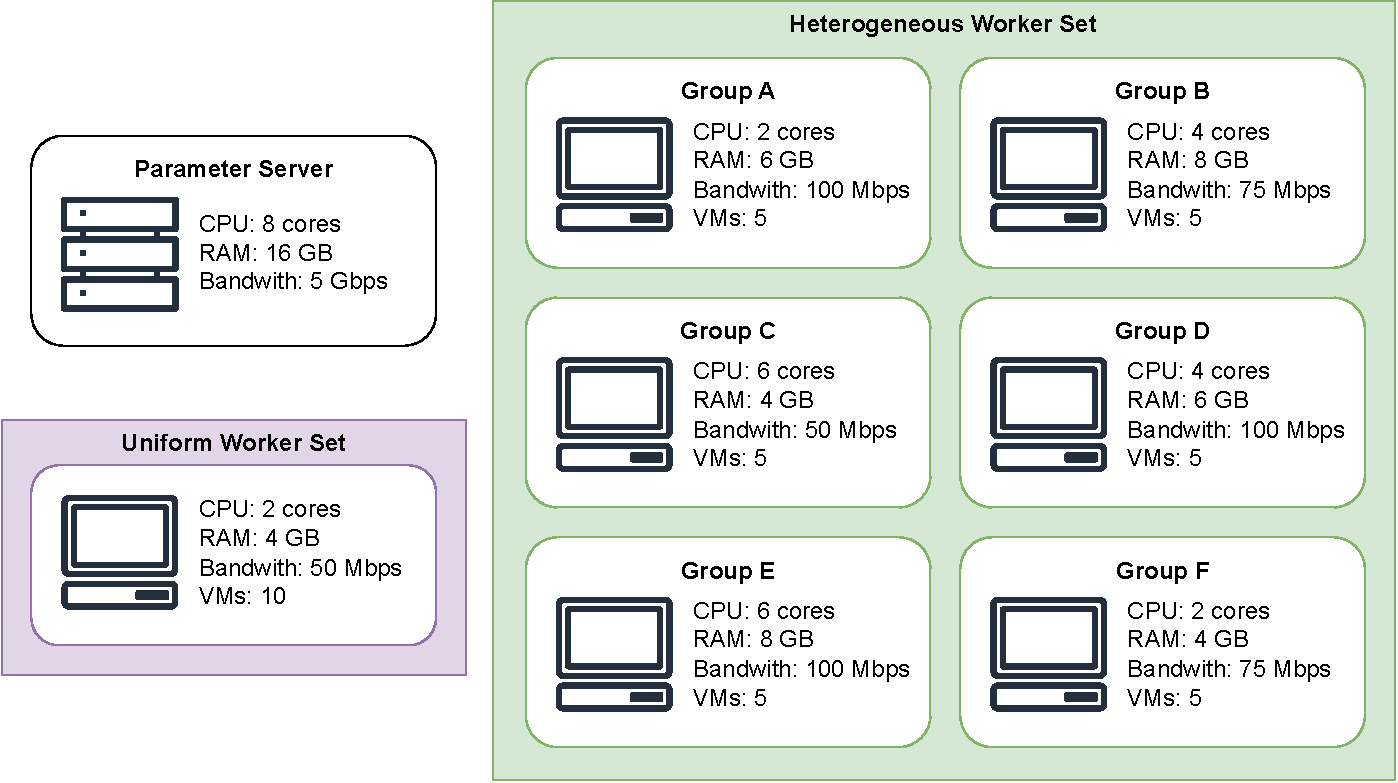
\includegraphics[width=\textwidth]{figs/vms.pdf}
    \caption[FL Testbed Configuration]{Illustration of the experimental setup, detailing the central Parameter Server and the two distinct sets of worker \acp{vm}: a uniform worker set with 10 \acp{vm}, and a heterogeneous worker set with 30 \acp{vm} comprising multiple groups with varying resource configurations.}
    \label{fig:experimental-setup}
\end{figure}


\section{Datasets and Models}
\label{sec:datasets-and-models}

Effective evaluation of a \ac{fl} framework requires careful selection of datasets and models relevant to its intended real-world applications. \ac{ids} and \ac{iot} environments stand out as highly practical and pertinent domains for \ac{fl} implementation. This is primarily due to the critical need for data privacy and security, alongside the inherent distributed nature of data sources in these settings. Training robust \ac{ids} models often necessitates access to sensitive data, like network traffic or device information, which is challenging or impossible to centralize \cite{10608461}.

\ac{fl} presents a viable solution by enabling collaborative model training among participants without requiring the sharing of raw data. Evaluating our framework within the context of \ac{ids} and \ac{iot} enables us to demonstrate its capabilities in scenarios that directly reflect these practical constraints and opportunities.

While well-established datasets like KDD98~\cite{kdd98}, KDDCUP99~\cite{kdd99}, or NSLKDD~\cite{nslkdd} exist for training \ac{ids} models, they are widely regarded as outdated and not fully representative of today's network traffic, as detailed in~\cite{kostas2023iotgem}. This significantly restricts their applicability to contemporary network security research. Considering this limitation, we decided to use two recent and widely-recognized state-of-the-art datasets, UNSW-NB15~\cite{unswnb15} and ToN-IoT~\cite{toniot}, which better capture current network threats and reflect \ac{iot} environments.

\subsection{UNSW-NB15}
\label{sec:unsw-nb15}

The UNSW-NB15 dataset is synthetically generated from the \ac{accs}. It combines real modern regular network traffic with synthesized contemporary attack activities. The dataset comprises over 2 million records, each with 49 features, and is suitable for both binary and multi-class classification tasks. Malicious activities are labeled with one of nine specific attack categories: \ac{dos}, Analysis, Backdoor, Exploits, Fuzzers, Generic, Reconnaissance, Shellcode, and Worms.

To avoid complex preprocessing procedures, in this study, we used the NF-UNSW-NB15\footnote{\url{https://espace.library.uq.edu.au/view/UQ:ffbb0c1}} preprocessed dataset published in~\cite{nfunswnb15} by the University of Queensland. This dataset version incorporates the same data as the original but standardizes features using NetFlow. NetFlow is a widely adopted Cisco protocol for collecting IP traffic information and monitoring network flow (e.g., total bytes transferred, number of packets, duration). The creators of this version state that their motivation was the lack of a standard feature set commonly found in general \ac{ids} datasets.

Following prior work on this dataset, specifically~\cite{abou2020evaluation}, which investigated various \acp{nn} including \ac{ann}, \ac{cnn}, and \ac{rnn} and found them to achieve similar results, we selected the \ac{ann} model. The \ac{ann} strikes a good balance between performance and computational efficiency, making it a suitable choice for potentially resource-limited \ac{fl} workers. However, this \ac{ann} model is rather small, in \cite{abou2020investigating} the authors used a larger model that we considered a better fit for our experiments. 

The \ac{ann} model used in this study consists of three hidden layers (300, 100, and 50 neurons) using the \ac{relu} activation function and a softmax for the output layer as shown in Figure~\ref{fig:unws_nn}. 

\begin{figure}[!htb]
    \centering
    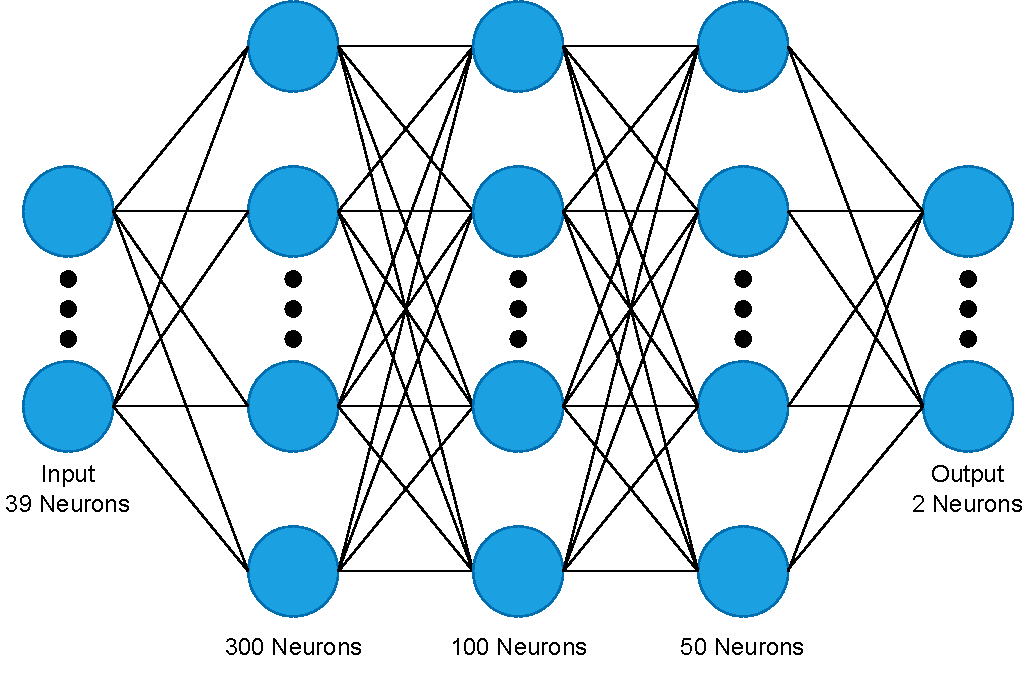
\includegraphics[width=0.8\textwidth]{figs/unsw_nn.pdf}
    \caption[UNSW-NB15 dataset model architecture]{Architecture of the ANN model used for the UNSW-NB15 dataset, consisting of three hidden layers with 300, 100, and 50 neurons, respectively.}
    \label{fig:unws_nn}
\end{figure}

\subsection{ToN-IoT}
\label{sec:ton-iot}

The ToN-IoT is a heterogeneous dataset created by the  \ac{accs} and released in 2019, specifically designed to include telemetry data from an \ac{iot} network. Generated on a realistic testbed, it provides various traces of \ac{iot} services, network traffic, and operating system logs. The dataset contains over 13 million samples and numerous attack scenarios, including Backdoor, \ac{dos}, \ac{ddos}, Injection, \ac{mitm}, Password, Ransomware, Scanning, and \ac{xss}. Like UNSW-NB15, ToN-IoT supports both multi-class attack classification and binary normal/malicious classification.

For this study, we used the NetFlow version of the ToN-IoT dataset, NF-ToN-IoT\footnote{\url{https://espace.library.uq.edu.au/view/UQ:38a2d07}}, published by the same authors as the NF-UNSW-NB15 dataset.

Based on the model evaluations for the ToN-IoT dataset presented in~\cite{kumar2021p2idf}, which compared a \ac{sae} and an \ac{ann} model, we selected the \ac{ann} model. The \ac{ann} architecture used for this dataset features two hidden layers with 32 and 16 neurons, respectively, also employing the \ac{relu} activation function and a softmax for the output layer. Dropout layers with a rate of 0.2 were included after each hidden layer. The model was trained using the Adam optimizer, mirroring the approach in the cited paper.

This model is smaller than the one used for UNSW-NB15, allowing it to exhibit distinctive characteristics and ensuring that the experiments are not biased by the model size. The architecture of the \ac{ann} model used for the ToN-IoT dataset is shown in Figure~\ref{fig:ton_nn}.

\begin{figure}[!htb]
    \centering
    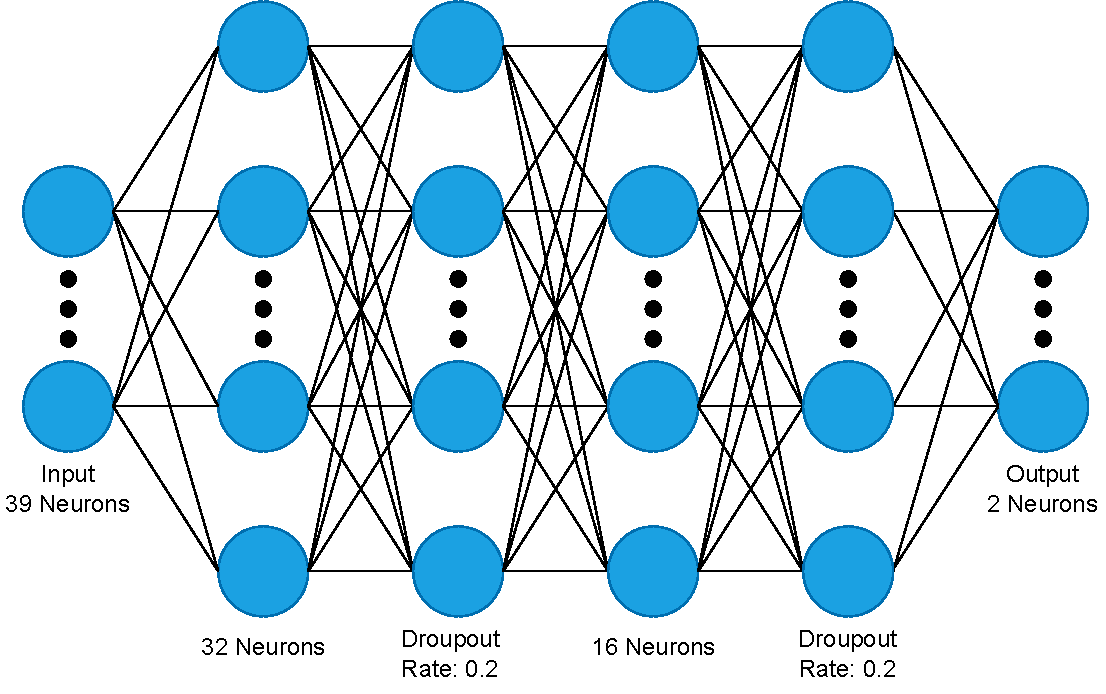
\includegraphics[width=0.9\textwidth]{figs/ton_nn.pdf}
    \caption[ToN-IoT dataset model architecture]{Architecture of the ANN model used for the ToN-IoT dataset, consisting of two hidden layers with 32 and 16 neurons, respectively, with dropout layers in between.}
    \label{fig:ton_nn}
\end{figure}

\subsection{Data Division}
\label{sec:data-division}

Our experiments focused on the binary classification task using the UNSW-NB15 and ToN-IoT datasets, aiming to train models that can distinguish between normal and malicious network traffic. To prepare the data for the distributed training process, we first preprocessed the datasets, without data normalization, and split them into three primary partitions: a training set (70\%), a validation set (15\%), and a testing set (15\%) for the UNSW-NB15 dataset, and a training set (90\%), a validation set (5\%), and a testing set (5\%) for the ToN-IoT dataset, because this dataset is significantly larger than UNSW-NB15 (over 13 million samples compared to UNSW-NB15's 2 million). This division ensures that the model can be trained effectively while also being evaluated on unseen data.

The training data were then partitioned among the workers participating in each experiment's subpool according to specific distribution strategies, primarily \ac{iid}, achieved by globally shuffling the dataset and distributing equal-sized partitions to each worker. A critical aspect of this data handling, consistent with the principles of \ac{fl} and preserving data privacy, is that each worker node performed data normalization (e.g., scaling features) using only the statistics (such as mean and standard deviation) derived from its own local data split, without sharing raw data or statistics with other nodes or the Parameter Server.

In this \ac{fl} setup, the validation set was used by the parameter server for periodic evaluation of the global model's performance throughout the training process. It is important to note that, for our experiments, the validation data was not used to influence the aggregation mechanism or global model updates, thereby ensuring the reported metrics effectively represent the model's generalization performance on unseen data, akin to a test set. The remaining testing sets were reserved for future evaluation of the final trained model's performance on unseen data.

Furthermore, the resilience mechanisms integrated into the system, such as handling client dropouts, do not alter the aggregation logic or influence the model update process. This ensures consistency and integrity in the training dynamics. Nonetheless, the modular design of the FL Backend does allow for future integration of validation-aware aggregation strategies. 




\section{Metrics}
\label{sec:metrics}


Rigorous evaluation of a \ac{ml} framework, particularly one designed for distributed and potentially unreliable environments like \ac{fl}, needs a comprehensive set of metrics. These metrics fall into two main categories: standard \ac{ml} performance metrics and system-level metrics derived from detailed logging.

Regarding the \ac{ml} performance, the specific metrics evaluated depend on the type of task being performed (classification or regression) and the loss function used. For the binary classification tasks utilizing the UNSW-NB15 and ToN-IoT datasets in this study, the following standard classification metrics are evaluated: \ac{mcc}, Accuracy, and F1-score \cite{chicco2020advantages, diallo2024machine}. They serve as primary indicators of the model's learning progress, convergence, and final quality.

Accuracy provides the overall proportion of correct predictions, while the F1-score offers a balanced view of precision and recall, which is particularly important for tasks like intrusion detection, where both minimizing false positives and false negatives is crucial. \ac{mcc} is a single-value metric that measures the quality of binary classifications, particularly useful for imbalanced datasets. It takes into account all four values in the confusion matrix: \ac{tp}, \ac{tn}, \ac{fp}, and \ac{fn}. It is calculated as:

\begin{equation}
    \text{MCC} = \frac{\text{TP} \cdot \text{TN} - \text{FP} \cdot \text{FN}}{\sqrt{(\text{TP} + \text{FP})(\text{TP} + \text{FN})(\text{TN} + \text{FP})(\text{TN} + \text{FN})}}
\end{equation}

For completeness and to demonstrate the framework's versatility beyond classification, standard regression metrics such \ac{smape}, \ac{mse}, and \ac{mae} \cite{chicco2021coefficient} are also considered as potential evaluation criteria depending on the model and dataset used. \ac{mse} is the average of the squared differences between predicted and actual values, and \ac{mae} is the average of the absolute differences. \ac{smape} is a measure of prediction accuracy, expressed as a percentage, calculated as:

\begin{equation}
    \text{SMAPE} = \frac{1}{n} \sum_{i=1}^{n} \frac{|y_i - \hat{y}_i|}{|y_i| + |\hat{y}_i|} \times 100
\end{equation}
Where \(y_i\) is the actual value, \(\hat{y}_i\) is the predicted value, and \(n\) is the number of data points.

For this evaluation, we primarily focused on global model validation metrics to assess the framework's overall convergence and generalization capabilities on unseen data, rather than tracking training metrics from individual clients. This choice was made to avoid additional overhead, and more importantly, because local training metrics in a federated setting, especially under \ac{non-iid} data distributions, can be misleading and do not reliably reflect the global model's learning progress. In such scenarios, client-specific metrics often exhibit high variance and are not indicative of the model's ability to generalize, making global validation performance a more meaningful and consistent measure.

In addition to model performance, evaluating the framework's resilience, scalability, and efficiency requires collecting detailed system-level data. As discussed in Section~\ref{sec:results-saving}, the framework generates comprehensive \ac{jsonl} log files for each node (Parameter Server and Workers). 

These logs capture a rich stream of events and data points throughout the experiment, including timestamps for send and receive operations of messages, details about exchanged payloads including size and type, epoch-level training and validation metrics (loss, accuracy, etc.), worker computation times for local training tasks, encode and decode times for messages, events indicating when workers join or leave the network, events indicating when workers fail, and markers for the start and end of the entire training run.

This detailed logging allows for the measurement and analysis of various system performance aspects, including the total run duration of the experiment, the evolution of loss and other \ac{ml} metrics over epochs, the number of messages sent and received and the total payload size exchanged, the total communication time across the network, and the total worker computation time and idle/wait time for both the Parameter Server and workers.

It also allows tracking and quantifying the types and timing of worker failures and their corresponding states during a round. This is crucial because it will enable us to differentiate between failures that halt progress (critical failures) and those that are less disruptive (non-critical failures). This provides empirical evidence for the framework's resilience claim by demonstrating how well it continues to train despite various failure scenarios. A worker's status during a round can be categorized into one of five states:

\begin{enumerate}[label=\roman*)]
    \item \textbf{Idle without fail:} The worker was available and did not experience a failure event while idle waiting for a task or the next round.
    \item \textbf{Worked successfully without failing:} The worker was assigned a local training task, completed it, and successfully communicated its update to the server without experiencing a failure event during this epoch.
    \item \textbf{Failed while idle:} A failure event occurred while the worker was available but not actively performing a local training task or communicating. This is generally less disruptive as no computation result is lost. This is considered a \textbf{non-critical failure} as the worker can rejoin the training process without any loss of contribution.
    \item \textbf{Failed while working:} A failure occurred while the worker actively performed a local training task or communicated their update. This is considered a \textbf{critical failure} as the ongoing computation or communication is interrupted, potentially requiring task reassignment in an asynchronous setting.
    \item \textbf{Failed after working successfully:} The worker completed its local training task and successfully communicated its update, but experienced a failure event afterward, before the start of the next round. This is considered a \textbf{non-critical failure} as the contribution for the current round was successfully made.
\end{enumerate}

These metrics provide insights into convergence speed and stability under different conditions, the impact of worker failures on training progress, communication overhead, and the overall efficiency of the framework. By analyzing these metrics, we can assess the framework's performance in terms of resilience, scalability, and efficiency, as well as its ability to adapt to varying worker capabilities and network conditions.



\section{Experimental Scenarios}
\label{sec:experimental-scenarios}

A series of experimental scenarios was designed and executed to comprehensively assess the performance, resilience, modularity, and scalability of the proposed Resilient Federated Learning Framework. These scenarios evaluate the framework's capabilities under different conditions, focusing on key aspects relevant to real-world \ac{fl} deployments, such as communication efficiency, fault tolerance, and scaling with a dynamic and heterogeneous worker pool. Three primary scenarios were investigated in this evaluation.

\textbf{Scenario 1: Impact of Communication Protocols and FL Algorithms} - This scenario is designed to measure and compare the communication overhead associated with different \ac{fl} algorithms implemented within the framework using the UNSW-NB15 dataset and aims to understand inherent communication costs. This is particularly important for identifying the most efficient approaches in bandwidth-limited environments, which are typical of edge computing scenarios where \ac{fl} is often applied. 

This scenario uses the first set of workers, consisting of 10 \acp{vm} with uniform specifications, connected to the Parameter Server. This setup allows for a controlled environment and better visualization of results. 

\textbf{Scenario 2: Resilience Evaluation under Worker Failures} - This scenario focuses on evaluating the framework's resilience mechanisms and their effectiveness in handling worker failures or disconnections across different communication protocols. By simulating worker failures while employing various communication protocols and training on the UNSW-NB15 dataset, we aim to assess how the framework maintains training continuity and performance. This scenario also uses the uniform worker set (10 \acp{vm}).

\textbf{Scenario 3: Scalability and Convergence with Large-Scale Failures} - This scenario evaluates the framework's scalability and overall robustness when operating with a larger and more heterogeneous worker pool while introducing simulated worker failures. By using both the uniform and heterogeneous worker sets (a total of 40 \acp{vm} with diverse specifications and network conditions) and conducting experiments with both the UNSW-NB15 and ToN-IoT datasets, this scenario provides a more realistic representation of a large-scale, dynamic \ac{fl} environment. The goal is to demonstrate that the framework can scale effectively and that the training process can still converge and achieve acceptable model performance despite numerous worker failures and disconnections.


In scenarios where failures were introduced, these were implemented as probabilistic worker failures occurring at different configured rates. Workers perform a graceful exit upon failure, attempting to rejoin the training process shortly after the failure event, mimicking realistic client behavior. This ensures that logs are saved and no results are lost.

Across these scenarios, a set of common hyperparameters and configurations was maintained to ensure consistency and comparability, while specific parameters were adjusted as needed for the targeted evaluation of each scenario. Table \ref{tab:hyperparameters} summarizes the common hyperparameters, which are fully tunable, used throughout the evaluation. These parameters are aligned with commonly adopted settings in state-of-the-art \ac{ml} training, ensuring the relevance and generalizability of our experimental results.

\begin{table}[!htb]
    \centering
    \caption[Core Hyperparameters for Experiments]{Core hyperparameters applied across the \ac{fl} experiments, representing a typical configuration used throughout the evaluation scenarios.}    \label{tab:hyperparameters}
    \begin{tabular}{Sc Sc}
        \toprule
        \textbf{Hyperparameter} & \textbf{Value} \\
        \midrule
        ML Backend & Keras with TensorFlow \\
        Optimizer & Adam \\
        Loss function & Categorical Crossentropy \\
        Batch size & 1024 \\
        Learning rate & 0.0001 \\
        Number of Epochs & 10 \\
        Local Epochs per worker & 3 \\
        Worker threshold & 50\% \\
        Workers per epoch & 70\% \\
        \bottomrule
    \end{tabular}
\end{table}

These scenarios, coupled with the detailed metric collection and analysis, provide a robust framework for evaluating the Resilient Federated Learning Framework's capabilities and validating its design principles against the challenges of real-world distributed environments.

All experimental results are publicly available on the framework's GitHub~\footnote{\url{https://github.com/leoalmPT/FlexFL/tree/dissertation}} repository for full transparency and reproducibility.



\section{Scenario 1: Impact of Communication Protocols and FL Algorithms}
\label{sec:scenario-1}

This scenario was designed to comprehensively evaluate the performance implications of selecting different communication protocols and \ac{fl} algorithms within the proposed framework. The primary goal is to quantify the communication overhead and execution times associated with various combinations, particularly highlighting how these factors interact in a controlled environment, such as the uniform worker setting, where network conditions are consistent across participants. 

This analysis is crucial for understanding the inherent performance characteristics of the framework's core components and informing appropriate protocol and algorithm choices for specific deployment environments, especially those with bandwidth or latency constraints typical of edge computing.

To achieve this, we tested all four implemented communication protocols: Zenoh, \ac{mqtt}, Kafka, and \ac{mpi}. These protocols were evaluated in conjunction with the four primary \ac{fl} algorithm paradigms supported by the framework: Centralized Synchronous, Centralized Asynchronous, Decentralized Synchronous, and Decentralized Asynchronous. 

It's important to recall the fundamental difference in communication patterns between Centralized and Decentralized \ac{fl}. Centralized approaches typically involve workers sending gradients to a central Parameter Server frequently. In a Centralized Synchronous setting, this aggregation occurs after a fixed number of worker batches have been processed, while in Centralized Asynchronous, the server processes updates from individual batches as they arrive.

Decentralized approaches, conversely, involve workers exchanging their full local models or weights less frequently, just once per training round or epoch. This distinction significantly impacts the volume and frequency of messages exchanged, potentially making Centralized approaches more susceptible to communication bottlenecks at the Parameter Server.

Furthermore, due to the design characteristics of the \ac{mpi} protocol, particularly its reliance on synchronous, blocking communication and lack of native support for a callback-based system, its evaluation was limited to the Decentralized Synchronous setting, to avoid incorrect time measurements and to ensure a fair comparison with the other protocols. Asynchronous communication is possible with \ac{mpi}, but it requires constant checking for incoming messages, adding considerable overhead. While this restricts a complete comparison across all algorithm types, it still serves as a valuable benchmark for evaluating the performance of other protocols, given its popularity in \ac{hpc}.

The performance was assessed using the metrics defined in Section~\ref{sec:metrics}: average communication time per worker, average working time per worker (local computation time), and average total run time for the entire experiment. The results presented here represent the average of three independent runs for each protocol-algorithm combination after a warmup run. These results are shown in Table~\ref{tab:scenario_1_messages} and Table~\ref{tab:scenario_1_times}.

\begin{table}[!htb]
    \centering
    \caption[Average Communication Volume in Scenario 1]{Average communication volume metrics, including the number of messages and total payload size per worker, for various communication protocols and \ac{fl} approaches evaluated in Scenario 1.}
    \label{tab:scenario_1_messages}
    \begin{tabular}{Sc Sc Sc Sc}
        \toprule
        \textbf{FL Approach} &
        \textbf{\begin{tabular}[c]{@{}c@{}}Comm\\Protocol\end{tabular}} &
        \textbf{\begin{tabular}[c]{@{}c@{}}Average Number\\Of Messages\end{tabular}} &
        \textbf{\begin{tabular}[c]{@{}c@{}}Average Total\\Payload Size (MB)\end{tabular}} \\
        \midrule
        \multirow{4.5}{*}{\begin{tabular}[c]{@{}c@{}}Decentralized\\Synchronous\end{tabular}}
        & MPI & $17.4\pm0.932$ & $2.71\pm0.164$ \\
        & Zenoh & $17.4\pm0.932$ & $2.71\pm0.164$ \\
        & MQTT & $17.4\pm0.932$ & $2.71\pm0.164$ \\
        & Kafka & $17.4\pm0.932$ & $2.71\pm0.164$ \\
        \midrule
        \multirow{3.5}{*}{\begin{tabular}[c]{@{}c@{}}Decentralized\\Asynchronous\end{tabular}}
        & Zenoh & $17.4\pm0.932$ & $2.71\pm0.164$ \\
        & MQTT & $17.4\pm0.932$ & $2.71\pm0.164$ \\
        & Kafka & $17.4\pm1.302$ & $2.71\pm0.229$ \\
        \midrule
        \multirow{3.5}{*}{\begin{tabular}[c]{@{}c@{}}Centralized\\Synchronous\end{tabular}}
        & Zenoh & $2285.4\pm2.044$ & $403.0\pm0.360$ \\
        & MQTT & $2285.4\pm1.935$ & $403.0\pm0.309$ \\
        & Kafka & $2285.4\pm1.069$ & $403.0\pm0.188$ \\
        \midrule
        \multirow{3.5}{*}{\begin{tabular}[c]{@{}c@{}}Centralized\\Asynchronous\end{tabular}}
        & Zenoh & $2285.4\pm1.302$ & $403.0\pm0.229$ \\
        & MQTT & $2285.4\pm1.975$ & $403.0\pm0.348$ \\
        & Kafka & $2285.4\pm1.302$ & $403.0\pm0.229$ \\
        \bottomrule
    \end{tabular}
\end{table}


\begin{table}[!htb]
    \centering
    \caption[Average Time Metrics in Scenario 1]{Average time metrics per worker, including communication time, working time, and total run time, for different communication protocols and \ac{fl} approaches evaluated in Scenario 1.}
    \label{tab:scenario_1_times}
    \begin{tabular}{Sc Sc Sc Sc Sc}
        \toprule
        \textbf{FL Approach} &
        \textbf{\begin{tabular}[c]{@{}c@{}}Comm\\Protocol\end{tabular}} &
        \textbf{\begin{tabular}[c]{@{}c@{}}Average Comm\\Time (s)\end{tabular}} &
        \textbf{\begin{tabular}[c]{@{}c@{}}Average Work\\Time (s)\end{tabular}} &
        \textbf{\begin{tabular}[c]{@{}c@{}}Average Total\\Run Time (s)\end{tabular}} \\
        \midrule
        \multirow{4.5}{*}{\begin{tabular}[c]{@{}c@{}}Decentralized\\Synchronous\end{tabular}}
        & MPI & $0.422\pm0.094$ & $83.92\pm13.54$ & $139.6\pm17.88$ \\
        & Zenoh & $0.097\pm0.021$ & $82.69\pm7.823$ & $136.7\pm5.091$ \\
        & MQTT & $0.115\pm0.022$ & $82.51\pm7.927$ & $138.1\pm8.274$ \\
        & Kafka & $1.705\pm0.213$ & $83.43\pm7.800$ & $139.9\pm4.286$ \\
        \midrule
        \multirow{3.5}{*}{\begin{tabular}[c]{@{}c@{}}Decentralized\\Asynchronous\end{tabular}}
        & Zenoh & $0.079\pm0.014$ & $82.45\pm8.541$ & $114.2\pm1.436$ \\
        & MQTT & $0.098\pm0.016$ & $82.71\pm7.866$ & $114.8\pm1.519$ \\
        & Kafka & $1.690\pm0.182$ & $83.20\pm7.322$ & $117.6\pm0.276$ \\
        \midrule
        \multirow{3.5}{*}{\begin{tabular}[c]{@{}c@{}}Centralized\\Synchronous\end{tabular}}
        & Zenoh & $23.35\pm5.524$ & $45.35\pm2.023$ & $269.2\pm1.609$ \\
        & MQTT & $25.39\pm3.492$ & $48.39\pm3.820$ & $250.9\pm26.09$ \\
        & Kafka & $360.3\pm2.206$ & $47.36\pm2.408$ & $1288.2\pm6.104$ \\
        \midrule
        \multirow{3.5}{*}{\begin{tabular}[c]{@{}c@{}}Centralized\\Asynchronous\end{tabular}}
        & Zenoh & $9.737\pm0.248$ & $47.19\pm2.287$ & $728.6\pm17.57$ \\
        & MQTT & $12.77\pm0.195$ & $46.58\pm2.796$ & $744.2\pm15.76$ \\
        & Kafka & $253.8\pm3.879$ & $48.37\pm2.251$ & $1865.0\pm19.69$ \\
        \bottomrule
    \end{tabular}
\end{table}


\subsection{Federated Learning Algorithms Comparison}
\label{sec:fl-algorithm-comparison}

% Decentralized Async avoid straggler problem from Decentralized Sync 
As expected based on the principles mentioned earlier, the Decentralized Asynchronous approach consistently achieves a lower average total run time compared to the Decentralized Synchronous approach across all evaluated protocols (e.g., with Zenoh, 114 vs. 136 seconds, respectively). To illustrate this, Figure \ref{fig:ds_timeline} and Figure \ref{fig:da_timeline} show the timeline of the Decentralized Synchronous and Asynchronous approaches, respectively.

We can observe the in the first case the parameter server waits for all workers to finish their local training before aggregating the updates, while in the second case, the workers can send their updates to the parameter server as soon as they finish their local training, allowing for a more efficient use of resources, avoiding the straggler problem and reducing the overall training time.

\begin{figure}[!htb]
    \centering
    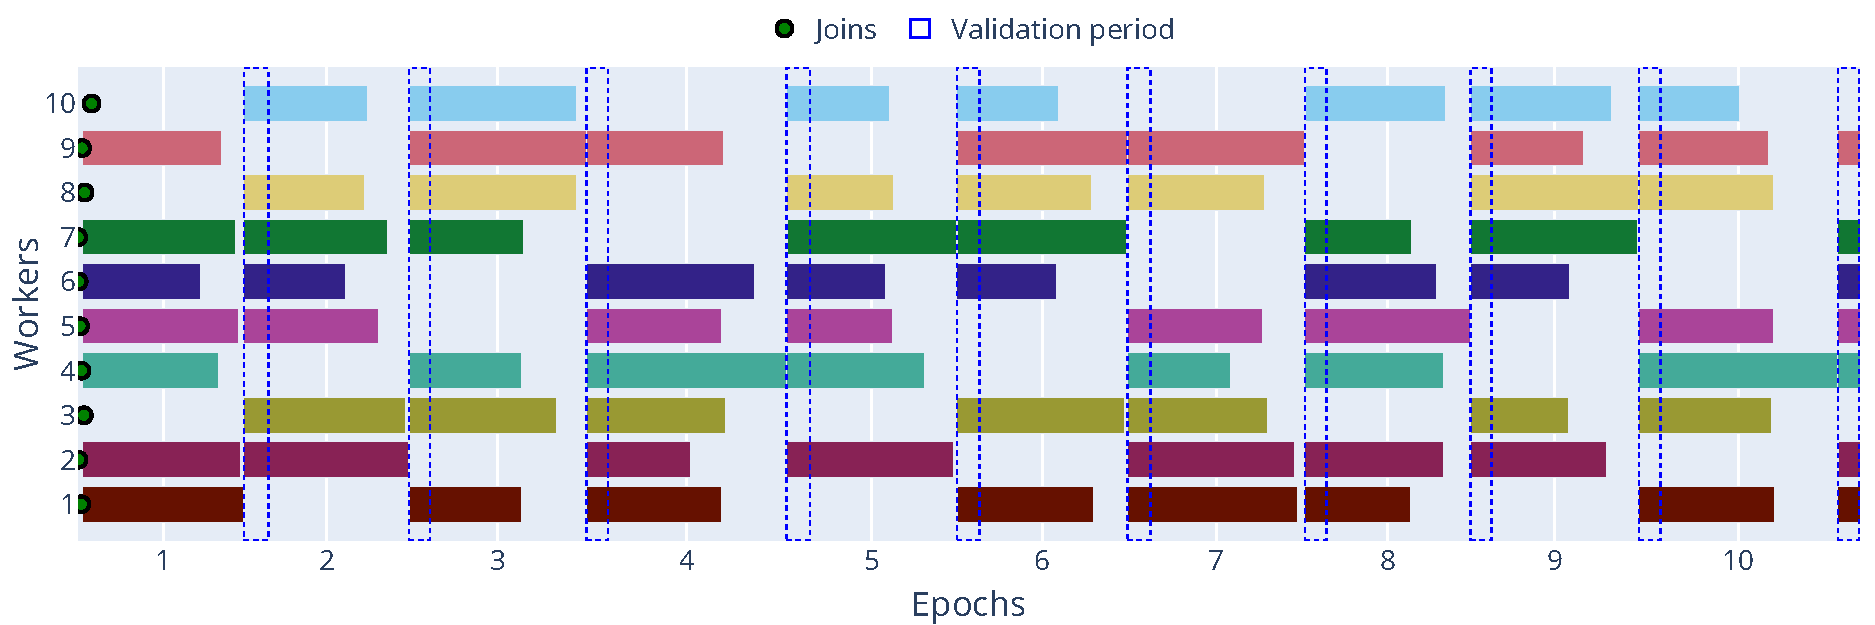
\includegraphics[width=\linewidth]{figs/scenario1/ds_timeline.pdf}
    \caption[Timeline of Decentralized Synchronous FL with Zenoh]{Timeline illustrating worker activity and idle periods across training epochs in the Decentralized Synchronous \ac{fl} approach with Zenoh, showing waiting for synchronization.}
    \label{fig:ds_timeline}
\end{figure}

\begin{figure}[!htb]
    \centering
    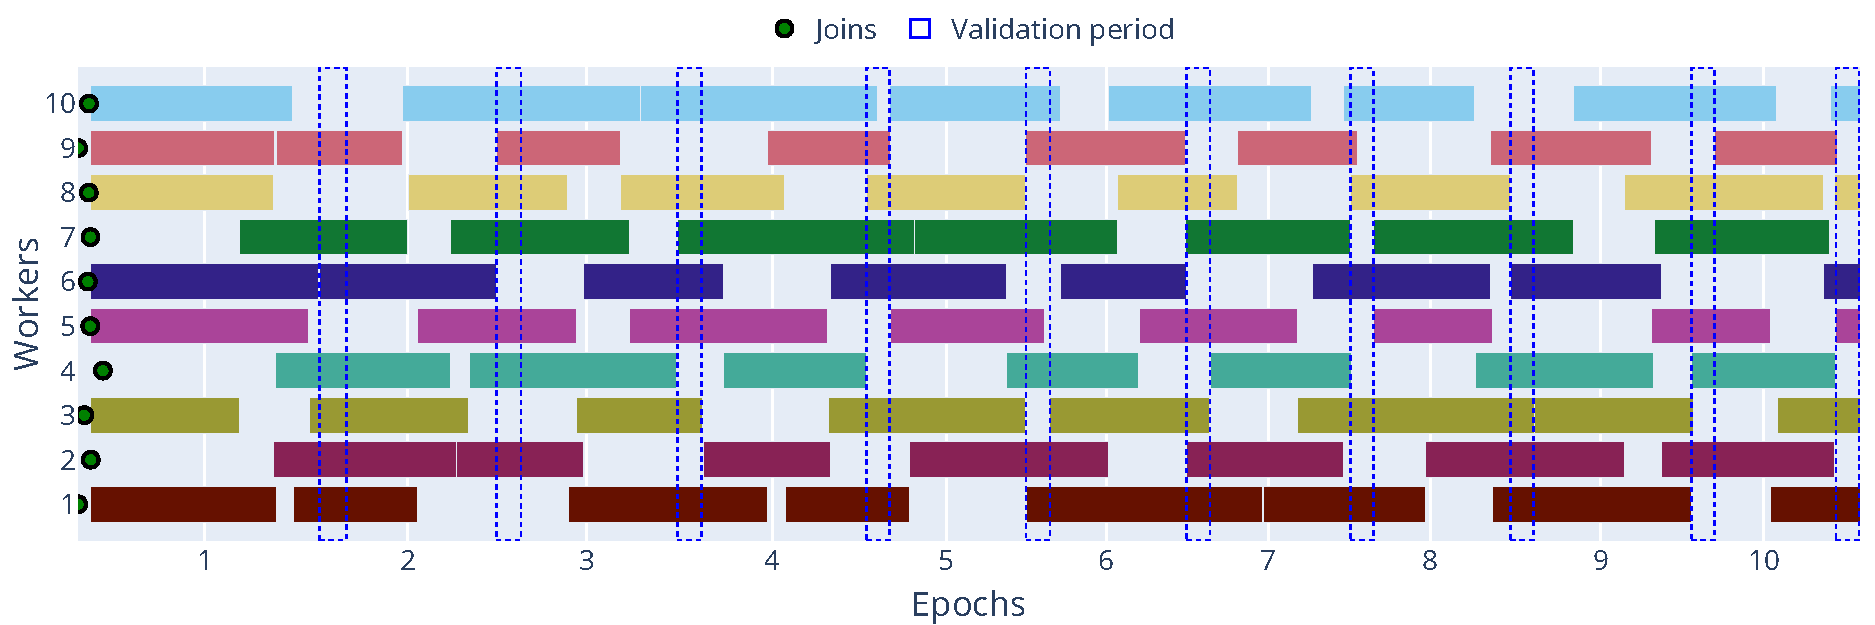
\includegraphics[width=\linewidth]{figs/scenario1/da_timeline.pdf}
    \caption[Timeline of Decentralized Asynchronous FL with Zenoh]{Timeline illustrating worker activity and idle periods across training epochs in the Decentralized Asynchronous \ac{fl} approach with Zenoh, demonstrating independent task completion and update submission.}
    \label{fig:da_timeline}
\end{figure}

This inherent advantage of asynchronous \ac{fl} is particularly critical in dynamic edge environments characterized by significant device heterogeneity, where worker speeds can vary drastically. When a worker joins, metadata is shared with the Parameter Server, this metadata can include information regarding their computational capabilities (e.g., CPU, memory, or GPU availability) and current network conditions (e.g., bandwidth and latency) and can be used in our modular Framework to implement more sophisticated scheduling policies to improve performance further. 

% Centralized has much more communication than Decentralized
As anticipated, Centralized methods involve a significantly higher frequency and volume of communication compared to Decentralized methods. For instance, across the Centralized experiments, the Parameter Server and workers exchanged a substantially larger number of messages (2285) and total payload size (403 MBs) compared to the Decentralized experiments, with 17 messages and a 2.7 MBs payload size.

% Centralized has much less local computation time than Decentralized - parameter server is doing the work and is a bottleneck 
We can also observe that workers in the Centralized approaches spend significantly less time on local computation compared to Decentralized workers. This discrepancy indicates that the server acts as a bottleneck in Centralized training, with workers spending considerable time idle or waiting for the server to aggregate updates and distribute the new global model, decreasing the local computation time from $\approx 83$ seconds in Decentralized approaches to $\approx 47$ seconds in Centralized approaches across all communication protocols.

% Centralized Asynchronous worse than Centralized Synchronous
This bottleneck effect was particularly noticeable in the Centralized Asynchronous setting, where the server must process every batch update from workers individually and immediately, potentially leading to increased server load and worker idle time, increasing the Total Run Time from 114 seconds in Decentralized Asynchronous with \ac{mqtt} to 744 seconds in the Centralized Asynchronous approach with the same communication protocol.

% Differences in payload size and number of messages
In asynchronous approaches, the number of messages exchanged and the total payload size vary from run to run, as reflected in standard deviations, due to the system dynamically adapting to worker availability. If a worker takes longer to complete their local training, other workers may complete more tasks, leading to a higher number of messages and a larger payload size. Conversely, in synchronous approaches, where workers proceed in lockstep, the number of messages and total payload size are expected to be the same across runs. 

This is the case for the Decentralized Synchronous approach, but not for the Centralized Synchronous approach. This is due to the number of iterations per epoch being determined by the total number of batches processed by the selected workers, if the dynamic worker pool selection results in different sets of workers (and thus potentially different total numbers of batches), it can introduce variability in the total number of iterations per round and consequently lead to varying numbers of messages and payload sizes.

\subsection{Communication Protocols Comparison}
\label{sec:communication-protocols-comparison}

% Overall overview of comm times
Observing the results in Table~\ref{tab:scenario_1_times}, distinct patterns emerge regarding the impact of the chosen communication protocol. Zenoh and \ac{mqtt} consistently exhibit lower average communication times across the tested \ac{fl} algorithm types compared to Kafka. Zenoh generally showed slightly lower communication times than \ac{mqtt}, although they were often closely comparable. 

\ac{mpi}, evaluated only in the Decentralized Synchronous context, showed higher communication times than Zenoh and \ac{mqtt} in that specific setting, and Kafka demonstrated the highest communication times across all paradigms where it was tested.

% Differences more evident in Centralized - more comm is done
This difference in communication performance is particularly evident when comparing the Centralized and Decentralized \ac{fl} approaches. Given the higher frequency and volume of communication, protocols with higher inherent latency, like Kafka, have a more pronounced negative impact on the overall communication time, achieving an average communication time of 360 seconds in the Centralized Synchronous compared to 23 and 25 seconds for Zenoh and \ac{mqtt}, respectively. 

% Similar working time - no comm overhead
In terms of average working time per worker, the communication protocol generally had a relatively similar impact across all protocols within the same \ac{fl} approach. This suggests that the time workers spend on local computation tasks is mainly independent of the communication method chosen, assuming the network does not become a severe bottleneck, completely halting progress. 

% parameter server comm in Sync approaches
Further analysis of Zenoh and \ac{mqtt} revealed that the average communication time was slightly higher in the Synchronous setting compared to the Asynchronous one. This observation suggests that the simultaneous arrival of synchronous updates from multiple workers at the central parameter server or broker might induce additional processing or queuing delays, which are then reflected in the increased communication time.

% Small std for times - stable runs, no significant outliers
Finally, analyzing the standard deviations across multiple runs provides valuable insights into the consistency and reliability of the framework's performance under different configurations. Low standard deviation values generally indicate that the experimental runs for a given configuration produced consistent results with no significant outliers, suggesting a stable and predictable behavior. 



\section{Scenario 2: Resilience Evaluation under Worker Failures}
\label{sec:scenario-2}


Building upon the foundational analysis of communication protocols and algorithms in Scenario 1, this scenario focuses specifically on evaluating the resilience mechanisms of the proposed Resilient Federated Learning Framework under simulated worker failures. The primary objective is to demonstrate the framework's ability to maintain training continuity and achieve model convergence even when individual worker nodes experience unexpected disconnections or failures.

The evaluation focused on the communication protocols best suited for dynamic and potentially unreliable network environments: Zenoh, \ac{mqtt}, and Kafka with the Decentralized Asynchronous \ac{fl} approach. This allows the training to proceed as long as there are active workers, processing updates as they arrive and naturally handling stragglers or failed nodes without waiting, by reassigning tasks and dynamically adapting to the available worker pool, which is crucial for resilience in dynamic environments.

To simulate worker failures, we introduced probabilistic failures into the system. Each worker was configured to have a certain probability of experiencing a failure event per second. We tested three different failure rates: 0.5\%, 1\%, and 3\% probability of failure per worker per second. 

When a failure occurred, the worker performed a graceful exit, simulating a planned shutdown or disengagement from the network, to ensure that logs are saved. Importantly, the framework was configured to allow failed workers to attempt to rejoin the training process shortly after the failure event, mimicking the behavior of real-world devices that might temporarily lose connectivity but eventually return.

To quantify the impact and handling of failures, we used the detailed system-level metrics, particularly focusing on the types of worker states described in Section~\ref{sec:metrics}:

\begin{itemize}
    \item \textbf{Non-critical failures:} These include \textit{iii: Failed while idle} and \textit{v: Failed after working successfully}. These failures are generally less disruptive as they do not interrupt an ongoing task that was assigned to the worker for the current round. The worker's contribution for the round, if any, was already submitted, or no task was missed.
    \item \textbf{Critical failures:} This refers to the \textit{iv: Failed while working} state, where a worker fails while actively performing its assigned task (local computation or communication). This type of failure is more disruptive as the partial or completed work for that task is lost, potentially requiring rescheduling or impacting the aggregation process, depending on the algorithm and framework's handling mechanisms.
\end{itemize}

Additionally, the other two states, \textit{i: Idle without fail} and \textit{ii: Worked successfully without failing}, are not directly related to failures but provide context for the worker's activity during the training process.

Table~\ref{tab:scenario-2-failures} presents a summary of the observed failure counts across the evaluated communication protocols and failure rates in the Decentralized Asynchronous setting.

\begin{table}[!htb]
    \centering
    \caption[Worker Failures in Decentralized Asynchronous FL]{Summary of observed worker failures during training with the Decentralized Asynchronous approach, detailing counts of non-critical, critical, and total failures, alongside the total run duration for each communication protocol and failure rate.}
    \label{tab:scenario-2-failures}
    \begin{tabular}{Sc Sc Sc Sc Sc Sc}
        \toprule
        \textbf{Failure Rate} &
        \textbf{\begin{tabular}[c]{@{}c@{}}Comm\\Protocol\end{tabular}} &
        \textbf{\begin{tabular}[c]{@{}c@{}}Non-Critical\\Failures\end{tabular}} &
        \textbf{\begin{tabular}[c]{@{}c@{}}Critical\\Failures\end{tabular}} &
        \textbf{\begin{tabular}[c]{@{}c@{}}Total\\Failures\end{tabular}} &
        \textbf{\begin{tabular}[c]{@{}c@{}}Total Run\\Duration (s)\end{tabular}} \\
        \midrule
        \multirow{3.5}{*}{\begin{tabular}[c]{@{}c@{}}0.5\% every\\Second\end{tabular}}
        & Zenoh & 3 & 5 & 8 & 123.3 \\
        & MQTT  & 2 & 6 & 8 & 125.0 \\
        & Kafka & 1 & 7 & 8 & 121.6 \\
        \midrule
        \multirow{3.5}{*}{\begin{tabular}[c]{@{}c@{}}1\% every\\Second\end{tabular}}
        & Zenoh & 3 & 10 & 13 & 123.8 \\
        & MQTT  & 2 & 12 & 14 & 129.5 \\
        & Kafka & 5 & 8  & 13 & 124.1 \\
        \midrule
        \multirow{3.5}{*}{\begin{tabular}[c]{@{}c@{}}3\% every\\Second\end{tabular}}
        & Zenoh & 8 & 30 & 38 & 149.4 \\
        & MQTT  & 2 & 38 & 40 & 155.7 \\
        & Kafka & 7 & 37 & 44 & 170.6 \\
        \bottomrule
    \end{tabular}
\end{table}

% All runs completed successfully
The results from this scenario provide strong empirical evidence for the framework's resilience. A key observation is that all experimental runs, regardless of the communication protocol or failure rate, completed successfully. This demonstrates that the framework's built-in mechanisms, such as the dynamic worker pool, task rescheduling for asynchronous approaches, and the Parameter Server's ability to handle sporadic updates, are effective in allowing the training process to continue and converge despite the presence of worker failures.

% Total number of failures increased with failure rate
As expected, the total number of observed failures increased significantly as the probabilistic failure rate was increased from 0.5\% to 3\%. While the runs for each configuration were initiated with the same random seed to promote consistency, slight variations in the exact number of failures occurred across different runs. 

% why same seed different values
This variability is inherent in the dynamic nature of the simulation, where factors such as the precise timing of failure events, the varying working times of individual workers, and the dynamic selection of workers for the subpool in each round can influence which workers are active and thus susceptible to failure at any given moment. 

% exaggerated failure rates as stress test
It is worth noting that a 1\% and 3\% failure rate per second represents an extremely chaotic and likely unrealistic scenario for most real-world deployments, serving as a stress test for the framework's robustness.

% higher run times - rescheduling
As anticipated, introducing failures led to a modest increase in the average total run time compared to the no-failure baseline. For the 0.5\% and 1\% failure rates, the increase was relatively small, varying with the training progress that needs to be rescheduled due to Critical Failures. 

% higher run times - pause training
However, at the 3\% failure rate, the increase in run time was more pronounced, this greater increase can be attributed not only to the higher volume of critical failures and subsequent task rescheduling but also to periods where the training process might have paused. The framework is designed to ensure a minimum number of active workers are available in each round to maintain training, if the dynamic worker pool drops below this threshold (7 workers or 70\% of the 10 workers), the parameter server pauses the training, by not sending new tasks and waits for enough workers to become available to proceed.

% visualizing results
To provide a deeper understanding of how failures were handled and their impact on the training process, we visualize the results through timelines, worker state matrices, and validation loss curves. Figure~\ref{fig:results_kafka}, Figure~\ref{fig:results_mqtt}, and Figure~\ref{fig:results_zenoh} illustrate the results for the Kafka, \ac{mqtt}, and Zenoh protocols, for the 0.5\%, 1\%, and 3\% failure rates, respectively. These visualizations offer a comprehensive overview of the behavior of various communication protocols under different failure scenarios.

\begin{figure}[!htb]
    \centering
    \begin{subfigure}[b]{\linewidth}
        \centering
        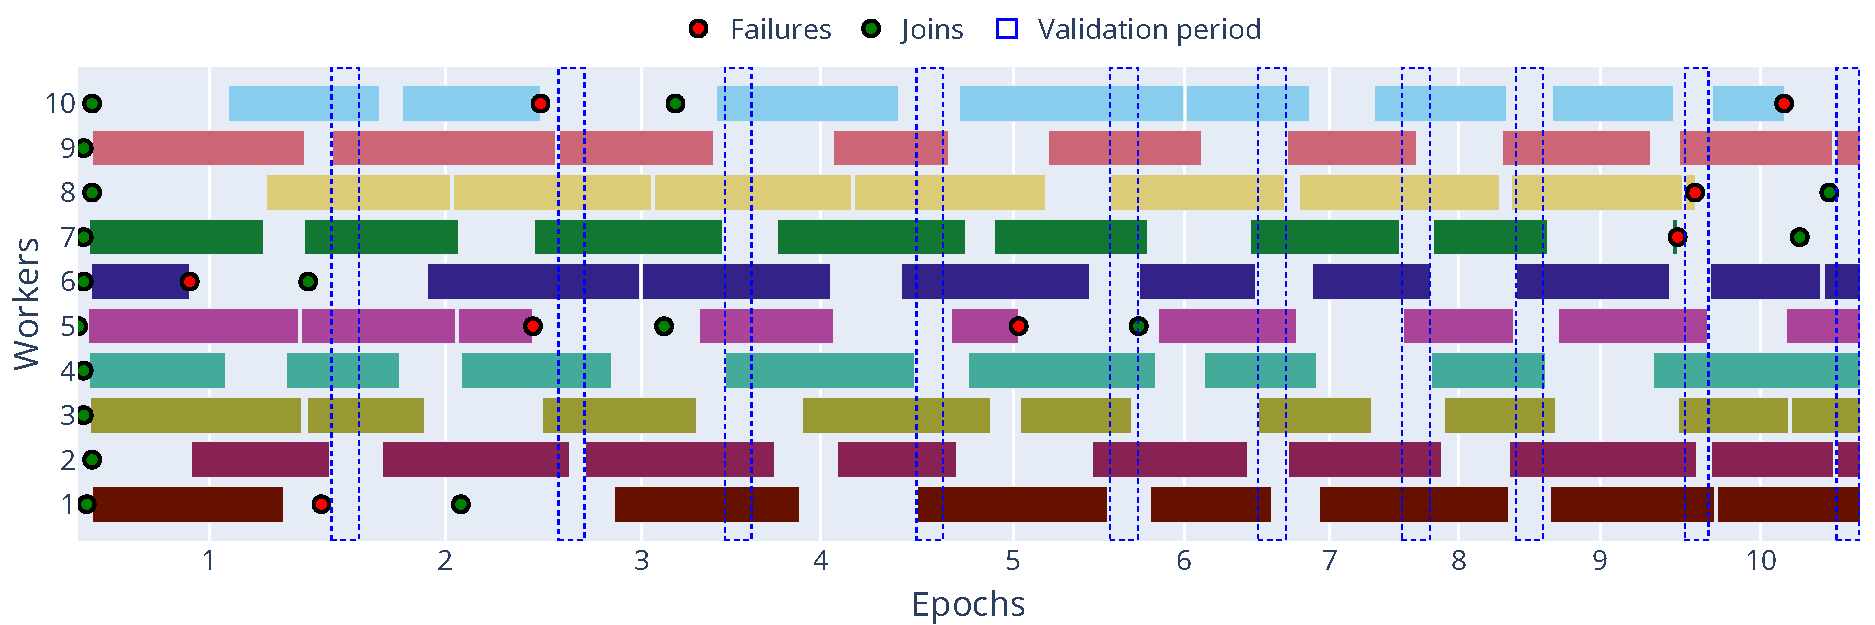
\includegraphics[width=\linewidth]{figs/scenario2/kafka_timeline.pdf}
        \caption{Timeline of worker activity and failure events.}
        \label{fig:timeline_kafka}
    \end{subfigure}
    \begin{subfigure}[b]{0.6\linewidth}
        \centering
        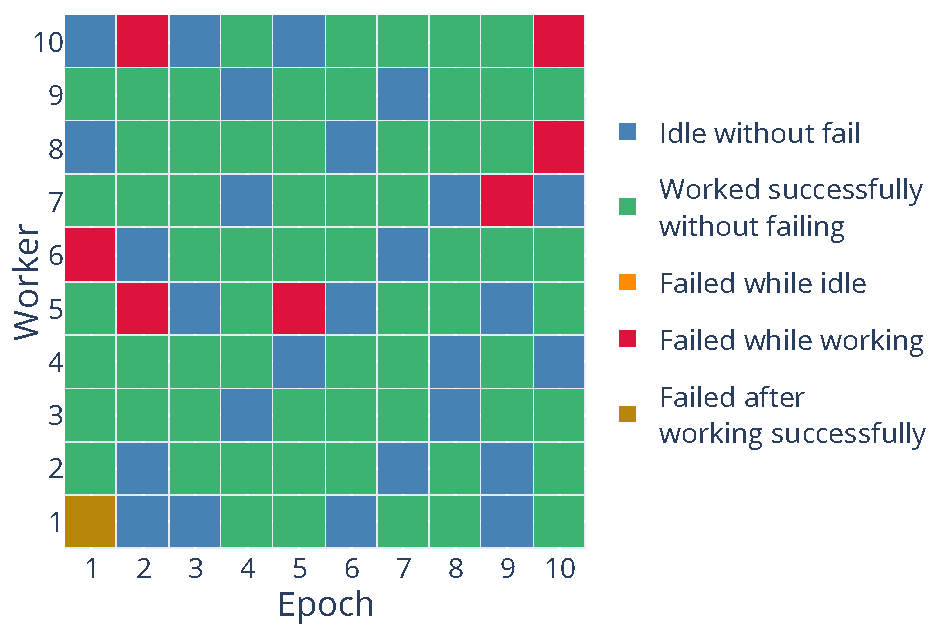
\includegraphics[width=\linewidth]{figs/scenario2/kafka_status.pdf}
        \caption{Worker state matrix across training epochs.}
        \label{fig:states_kafka}
    \end{subfigure}
    % \hfill
    \begin{subfigure}[b]{0.6\linewidth}
        \centering
        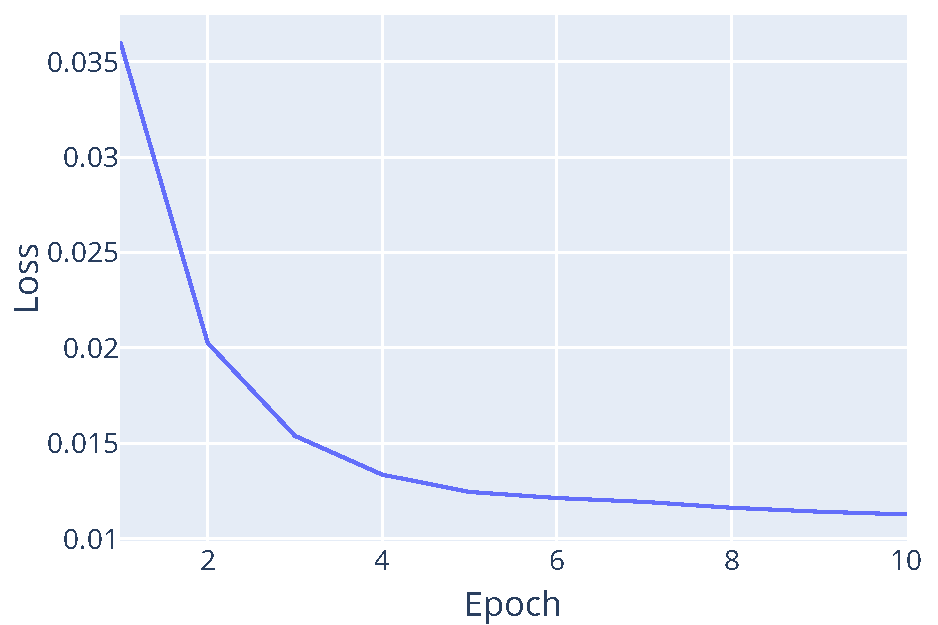
\includegraphics[width=\linewidth]{figs/scenario2/kafka_loss.pdf}
        \caption{Validation loss curve.}
        \label{fig:loss_kafka}
    \end{subfigure}
    \caption{Training results with the Kafka protocol (0.5\% failure rate).}
    \label{fig:results_kafka}
\end{figure}

\begin{figure}[!htb]
    \centering
    \begin{subfigure}[b]{\linewidth}
        \centering
        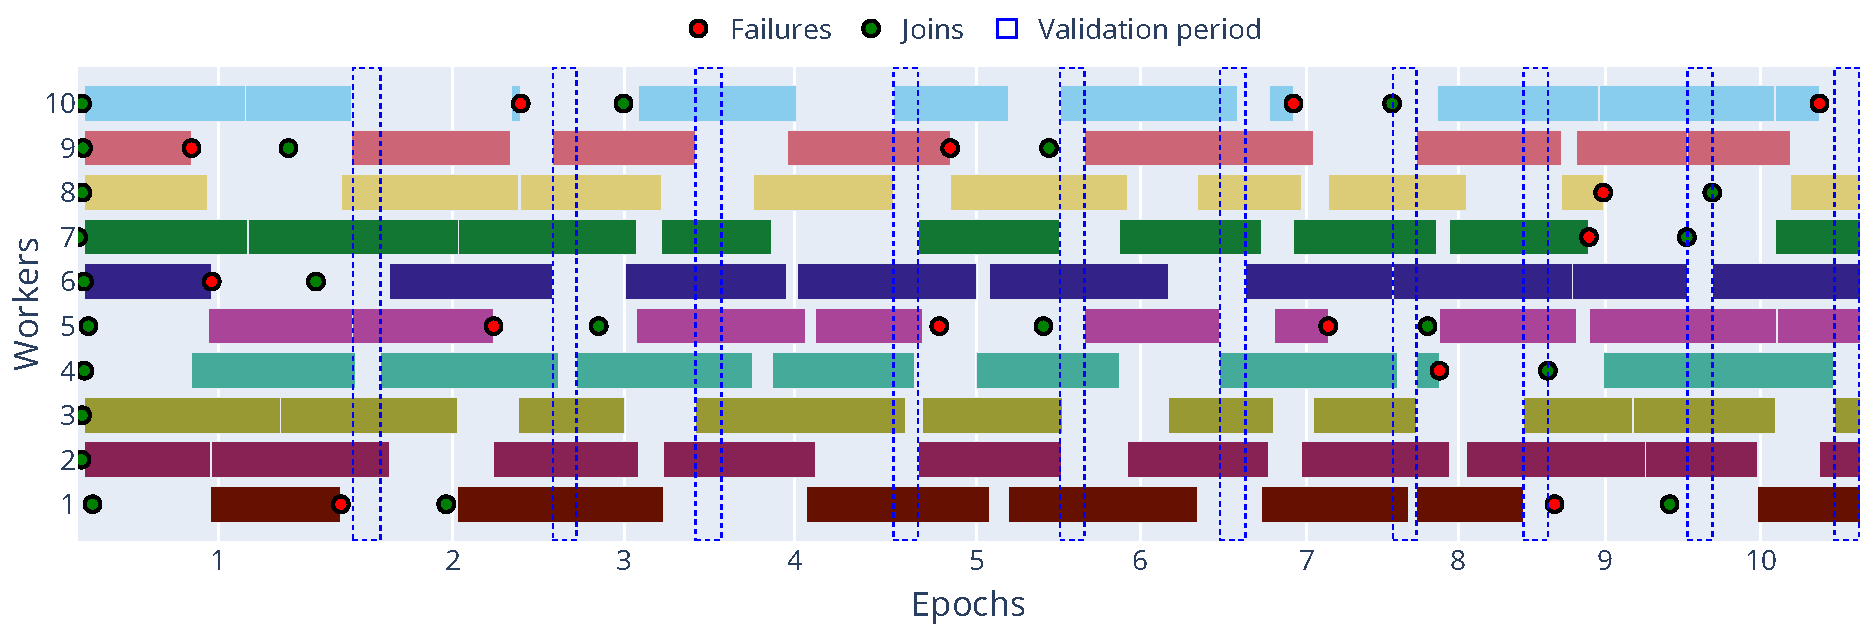
\includegraphics[width=\linewidth]{figs/scenario2/mqtt_timeline.pdf}
        \caption{Timeline of worker activity and failure events.}
        \label{fig:timeline_mqtt}
    \end{subfigure}
    \begin{subfigure}[b]{0.6\linewidth}
        \centering
        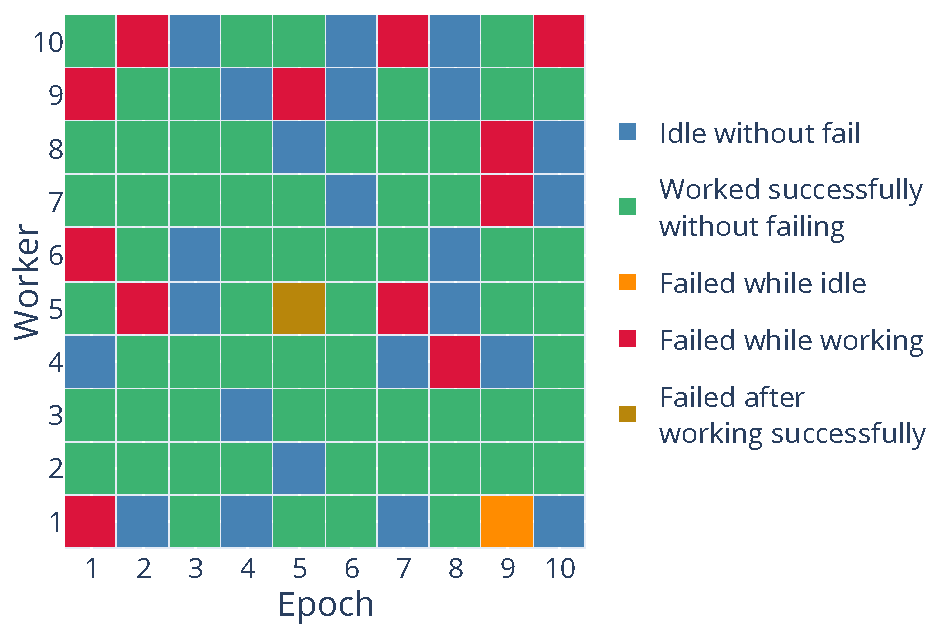
\includegraphics[width=\linewidth]{figs/scenario2/mqtt_status.pdf}
        \caption{Worker state matrix across training epochs.}
        \label{fig:states_mqtt}
    \end{subfigure}
    % \hfill
    \begin{subfigure}[b]{0.6\linewidth}
        \centering
        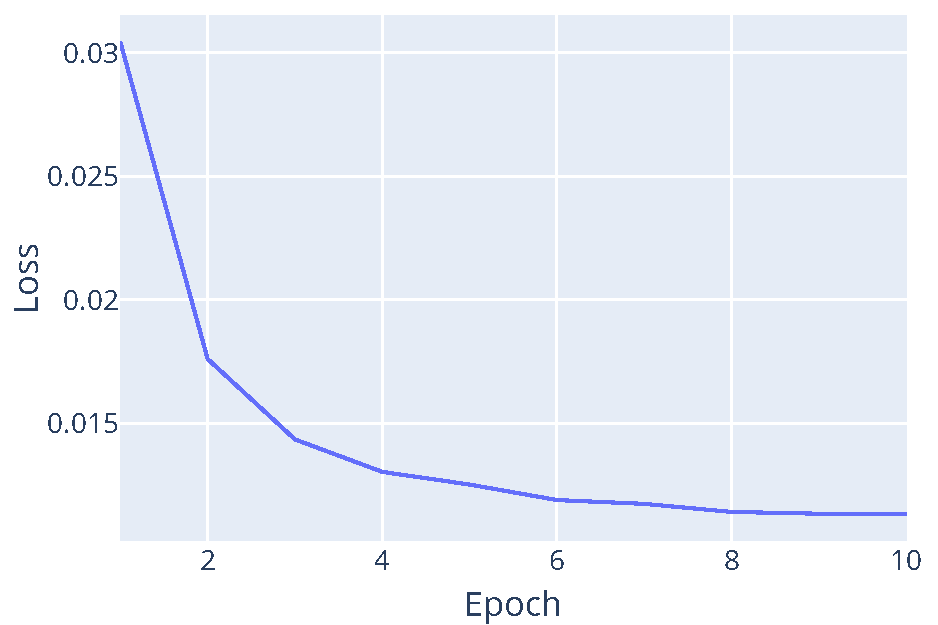
\includegraphics[width=\linewidth]{figs/scenario2/mqtt_loss.pdf}
        \caption{Validation loss curve.}
        \label{fig:loss_mqtt}
    \end{subfigure}
    \caption[]{Training results with the MQTT protocol (1\% failure rate).}
    \label{fig:results_mqtt}
\end{figure}

\begin{figure}[!htb]
    \centering
    \begin{subfigure}[b]{\linewidth}
        \centering
        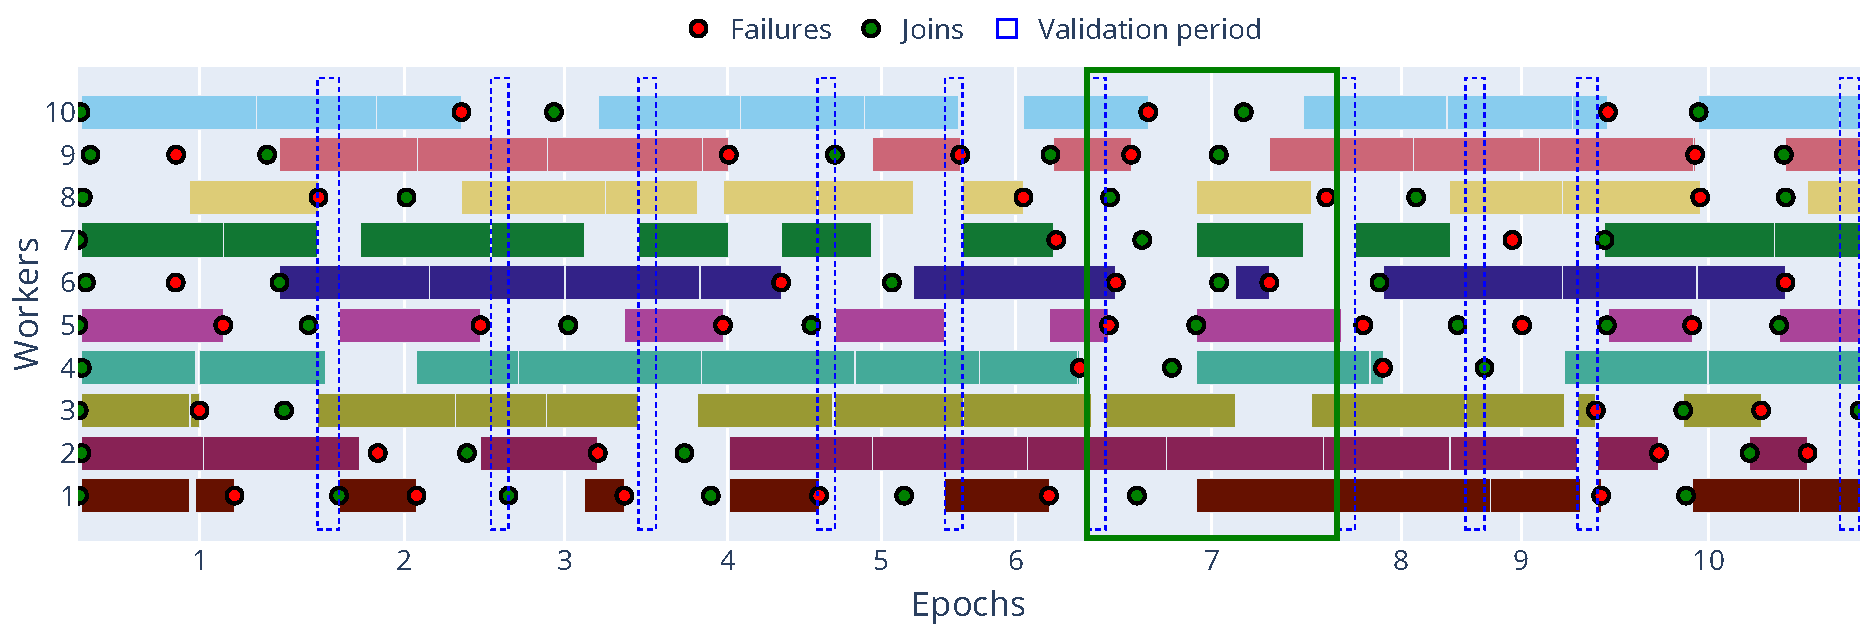
\includegraphics[width=\linewidth]{figs/scenario2/zenoh_timeline.pdf}
        \caption{Timeline of worker activity and failure events.}
        \label{fig:timeline_zenoh}
    \end{subfigure}
    \begin{subfigure}[b]{0.6\linewidth}
        \centering
        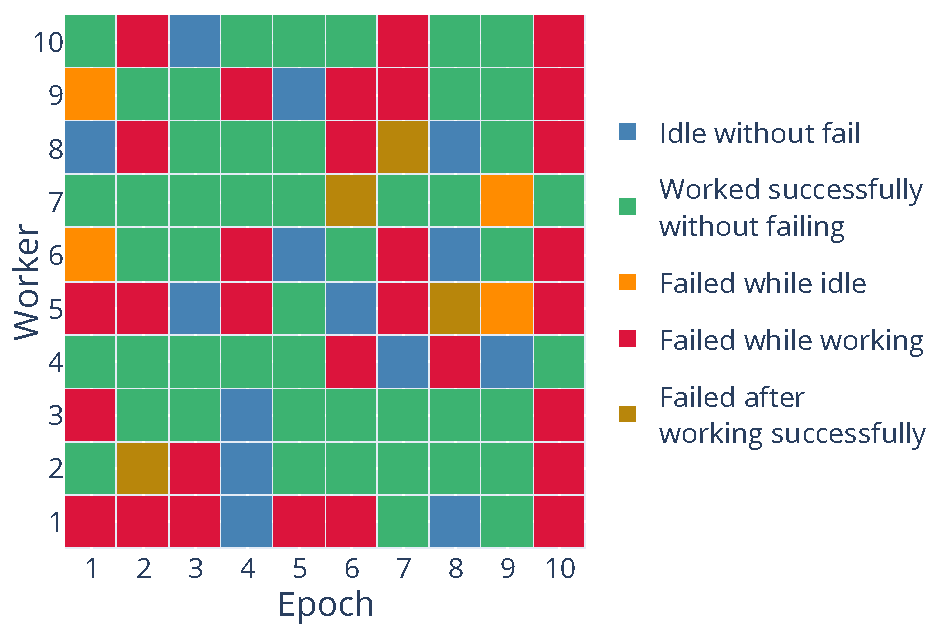
\includegraphics[width=\linewidth]{figs/scenario2/zenoh_status.pdf}
        \caption{Worker state matrix across training epochs.}
        \label{fig:states_zenoh}
    \end{subfigure}
    % \hfill
    \begin{subfigure}[b]{0.6\linewidth}
        \centering
        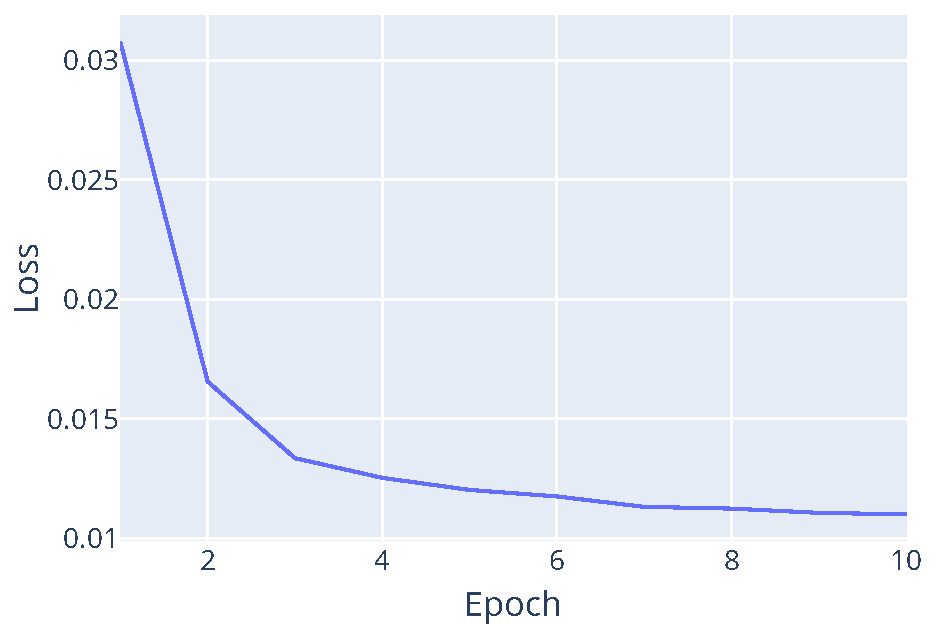
\includegraphics[width=\linewidth]{figs/scenario2/zenoh_loss.pdf}
        \caption{Validation loss curve.}
        \label{fig:loss_zenoh}
    \end{subfigure}
    \caption{Training results with the Zenoh protocol (3\% failure rate).}
    \label{fig:results_zenoh}
\end{figure}

% timelines and rescheduling 
We can observe that the timelines show the activity (working, idle) of each worker over time, clearly marking when failure events occurred and when workers rejoined the network. They also illustrate how the Parameter Server reacted to critical failures, such as rescheduling tasks in the Decentralized Asynchronous setting. Specifically, when a worker fails while working or finishes their task, the Parameter Server sends a new task to another worker as soon as possible, allowing the training to continue without significant delays.

% pause training
In cases where the number of active workers dropped below the threshold (7 workers), the Parameter Server paused the training until enough workers were available to proceed. This is evident in Figure~\ref{fig:timeline_zenoh} at epoch 7, as soon as the number of workers reached the threshold (when worker 5 joined), the parameter server resumed the training process by sending new tasks to 5 workers $\{1, 4, 5, 7, 8\}$, while 2 were already working on their tasks $\{2, 3\}$ and the remaining 3 workers were offline due to failures $\{6, 9, 10\}$.

% worker state matrices
The worker state matrices offer a clear, epoch-by-epoch view of each worker's state (Idle without fail, Worked successfully, Failed while idle, Failed while working, Failed after working successfully), making it easier to evaluate the frequency and type of failures experienced by individual workers throughout the experiment. 

% loss plots
Finally, plots showing the validation loss curve over epochs for representative runs (Kafka with 0.5\% failure rate, MQTT with 1\% failure rate, and Zenoh with 3\% failure rate) visually confirm that the model consistently converged, even under the highest simulated failure rate, demonstrating that the framework's resilience mechanisms effectively preserved the integrity of the training process and allowed the model to learn despite the disruptions.



\section{Scenario 3: Scalability and Convergence with Large-Scale Failures}
\label{sec:scenario-3}

This final scenario is designed to push the boundaries of the Resilient Federated Learning Framework by evaluating its scalability and overall robustness when operating with a significantly larger worker pool and simultaneously introducing substantial simulated failures. The objective is to demonstrate that the framework can effectively scale the training process and achieve model convergence even in a large-scale, dynamic \ac{fl} environment where numerous worker nodes are experiencing disruptions.

For this evaluation, we used the combined worker set, comprising both the uniform set (10 \acp{vm}) and the heterogeneous set (30 \acp{vm}), totaling 40 worker \acp{vm}. This configuration provides a more realistic representation of real-world \ac{fl} deployments, involving a diverse group of devices with varying computational capabilities and network conditions.

Given the significantly larger worker pool (40 \acp{vm} compared to 10 in previous scenarios), the total dataset was partitioned across a greater number of devices. Consequently, each worker had access to a smaller local data subset. To ensure robust model convergence and to adequately compensate for the reduced training data available per client in each round, the number of training epochs was increased from 10 to 20. This adjustment enables more global aggregation steps, which is crucial for achieving comparable model quality and convergence in environments with distributed and sparse data partitions.

Based on the findings from Scenario 1 and Scenario 2, we selected the Decentralized Asynchronous algorithm due to its inherent suitability for dynamic environments and resilience to failures, and the Zenoh communication protocol, which consistently exhibited lower communication overhead and native support for dynamic participant management. This combination is expected to be the most robust for large-scale, failure-prone scenarios.

The experiments in this scenario were conducted using both the UNSW-NB15 and ToN-IoT datasets. Evaluating the framework with two distinct datasets demonstrates its versatility and ability to handle different data characteristics and problem domains at scale. Both datasets were configured for the binary classification task, as described in Section~\ref{sec:datasets-and-models}, with data partitioned using the \ac{iid} strategy.

Simulated worker failures were introduced at a 1\% probabilistic failure rate per worker per second. This rate represents a significant level of churn and disruption across the 40 worker nodes, testing the framework's ability to maintain continuity under considerable stress.

Table~\ref{tab:scenario-3-failures} presents the average counts of non-critical, critical, and total failures observed across runs for each dataset at the 1\% failure rate.

\begin{table}[!htb]
    \centering
    \caption[Worker Failures and Run Time at 1\% Rate with 40 Workers]{Failure counts observed during training with the Decentralized Asynchronous approach and a 1\% failure rate with 40 workers, detailing non-critical, critical, and total failures, alongside the total run duration for both the UNSW-NB15 and ToN-IoT datasets.}
    \label{tab:scenario-3-failures}
    \begin{tabular}{Sc Sc Sc Sc Sc}
        \toprule
        \textbf{Dataset} &
        \textbf{\begin{tabular}[c]{@{}c@{}}Non-Critical\\Failures\end{tabular}} &
        \textbf{\begin{tabular}[c]{@{}c@{}}Critical\\Failures\end{tabular}} &
        \textbf{\begin{tabular}[c]{@{}c@{}}Total\\Failures\end{tabular}} &
        \textbf{\begin{tabular}[c]{@{}c@{}}Total Run\\Duration (s)\end{tabular}} \\
        \midrule
        UNSW-NB15 & 9 & 8 & 17 & 62.6 \\
        ToN-IoT & 20 & 27 & 47 & 122.5 \\
        \bottomrule
    \end{tabular}
\end{table}

% runs completed successfully
Similar to Scenario 2, all experimental runs in this scenario, for both datasets and with the 40-worker setup and 1\% failure rate, completed successfully. This further validates the framework's resilience mechanisms, which effectively managed the dynamic worker pool and allowed for continuous training despite the presence of numerous worker failures. This is a critical finding, demonstrating that the framework scales effectively and maintains its resilience properties even under increased load and disruption.

% run times - unsw comparison
Comparing the total run durations, for the UNSW-NB15 dataset, the total run duration of 62 seconds compared to 123 seconds in Scenario 2 with 10 workers and the same failure rate, this counter-intuitive result, despite the increased number of epochs (20 vs. 10), is primarily due to the data partitioning strategy. With 40 workers instead of 10, each worker processed approximately one-quarter of the total training data per local epoch. While the total number of global epochs doubled, the reduced local training time per worker per epoch, combined with the asynchronous nature of the algorithm, allowed for continuous progress without waiting for all stragglers, enabling a faster overall completion due to increased parallelization.

% run times - toniot
Conversely, the ToN-IoT dataset resulted in a significantly longer average total run duration of 122.5 seconds compared to UNSW-NB15 (62.6 seconds) in this scenario. As noted in Section~\ref{sec:datasets-and-models}, the ToN-IoT dataset is considerably larger than UNSW-NB15 (over 13 million samples versus 2 million), and despite the ToN-IoT model having a smaller architecture, the sheer volume of data in ToN-IoT requires more extensive local computation per worker, leading to a longer overall training duration.

To visually illustrate the training process at scale, Figures~\ref{fig:scenario3_unsw_results} and \ref{fig:scenario3_toniot_results} show the validation loss and other key epoch metrics over training epochs for a representative run for the UNSW-NB15 and ToN-IoT datasets, respectively.

\begin{figure}[!htb]
    \centering
    \begin{subfigure}[b]{0.49\linewidth}
        \centering
        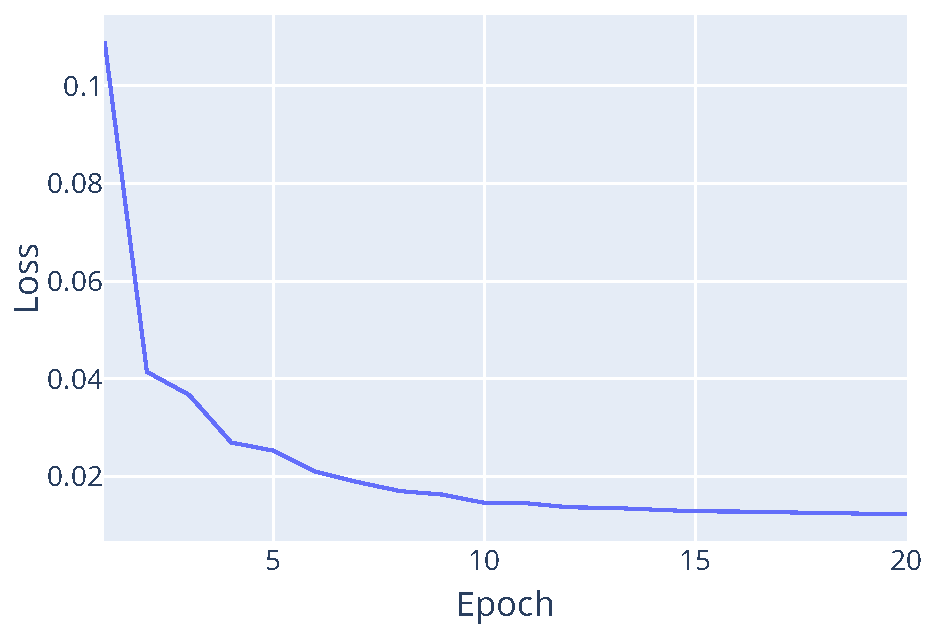
\includegraphics[width=\linewidth]{figs/scenario3/unsw_loss.pdf}
        \caption{Validation loss curve for UNSW-NB15 dataset.}
        \label{fig:scenario3_unsw_loss}
    \end{subfigure}
    \hfill
    \begin{subfigure}[b]{0.49\linewidth}
        \centering
        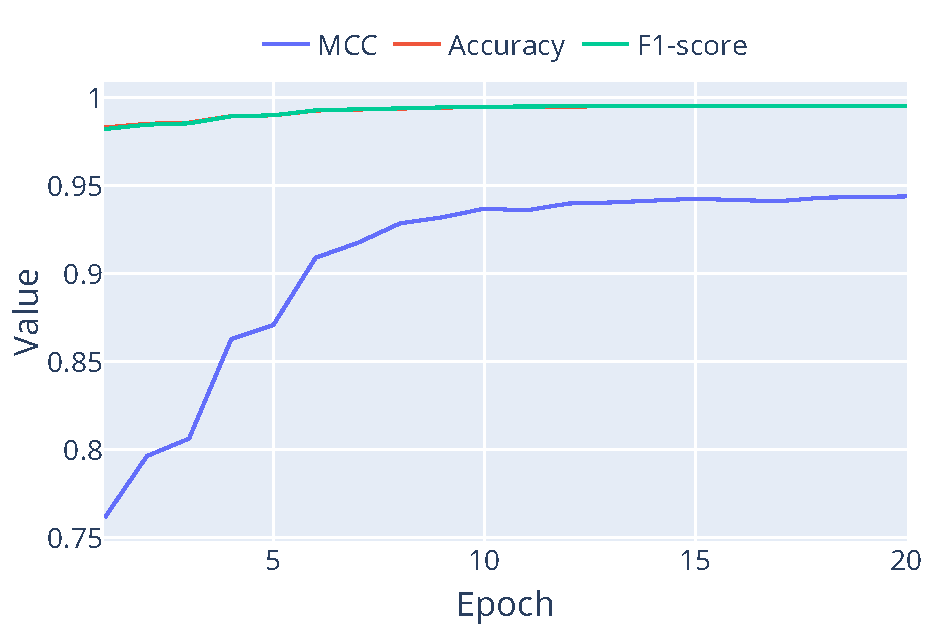
\includegraphics[width=\linewidth]{figs/scenario3/unsw_metrics.pdf}
        \caption{Epoch metrics for UNSW-NB15 dataset.}
        \label{fig:scenario3_unsw_metrics}
    \end{subfigure}
    \caption[UNSW-NB15 Training Results with Decentralized Asynchronous FL]{Training results with the UNSW-NB15 dataset using Decentralized Asynchronous approach and Zenoh protocol with 40 workers and 1\% failure rate.}
    \label{fig:scenario3_unsw_results}
\end{figure}

\begin{figure}[!htb]
    \centering
    \begin{subfigure}[b]{0.49\linewidth}
        \centering
        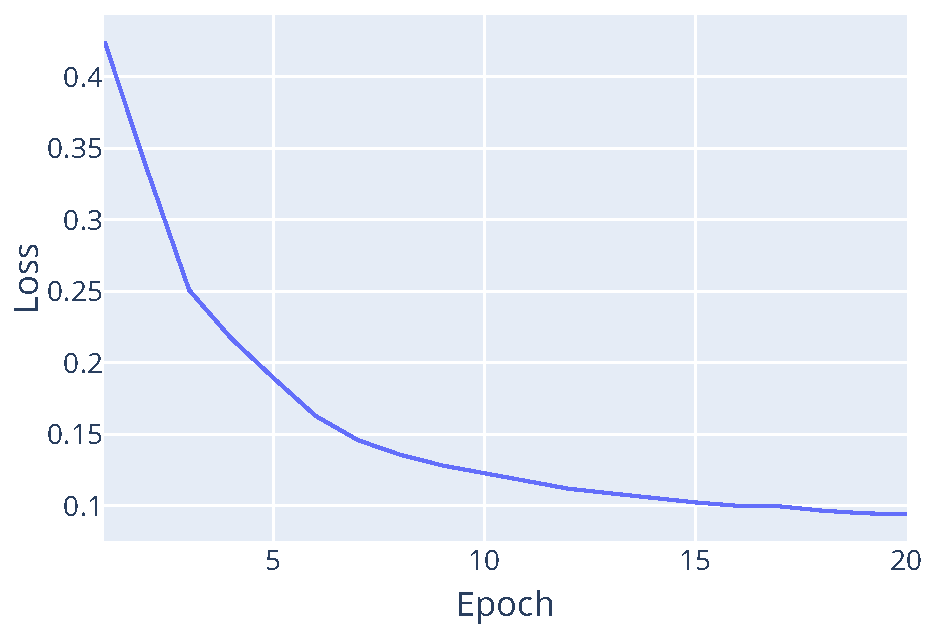
\includegraphics[width=\linewidth]{figs/scenario3/toniot_loss.pdf}
        \caption{Validation loss curve for ToN-IoT dataset.}
        \label{fig:scenario3_toniot_loss}
    \end{subfigure}
    \hfill
    \begin{subfigure}[b]{0.49\linewidth}
        \centering
        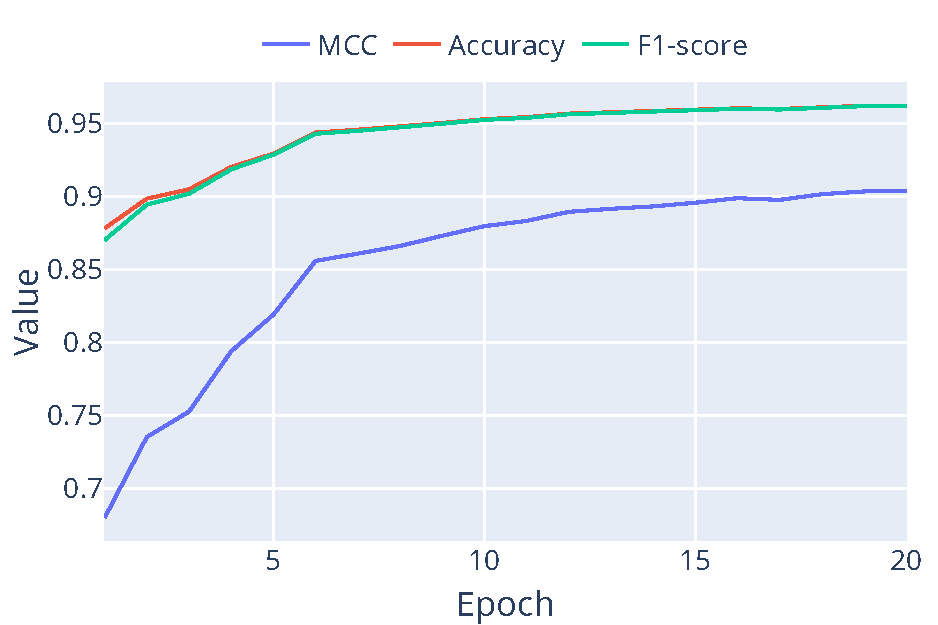
\includegraphics[width=\linewidth]{figs/scenario3/toniot_metrics.pdf}
        \caption{Epoch metrics for ToN-IoT dataset.}
        \label{fig:scenario3_toniot_metrics}
    \end{subfigure}
    \caption[ToN-IoT Training Results with Decentralized Asynchronous FL]{Training results with the ToN-IoT dataset using Decentralized Asynchronous approach and Zenoh protocol with 40 workers and 1\% failure rate.}
    \label{fig:scenario3_toniot_results}
\end{figure}

These plots provide visual confirmation of the framework's ability to maintain stable training and achieve model convergence even under the demanding conditions of Scenario 3, characterized by a large and heterogeneous worker pool and frequent simulated failures. 

For both datasets, the validation loss curves consistently decrease over epochs, indicating that the models are effectively learning and improving. Simultaneously, the MCC, Accuracy, and F1-score metrics exhibit a clear upward trend, converging towards high-performance values, which demonstrates the framework's robustness in ensuring model quality despite disruptions.

The successful completion of all runs in this challenging scenario, coupled with clear evidence of model convergence and high final performance metrics, validates the core design principles of the Resilient Federated Learning Framework. It proves its capability to effectively manage dynamic worker participation, tolerate significant node failures, and adapt to varying data and network conditions. 

For the UNSW-NB15 dataset, the final MCC achieved was 0.944, and for the ToN-IoT dataset, it was 0.903, further underlining the effectiveness of the training process even under adverse conditions. This comprehensive evaluation demonstrates that the framework is a robust and scalable solution for real-world Federated Learning deployments, particularly in edge computing environments where resilience and efficiency are paramount.
